
\documentclass[%
 aip,
 chaos,
 amsmath,amssymb,
 reprint,
]{revtex4-2}

\usepackage{graphicx}
\usepackage{subcaption}
\usepackage{booktabs}
\usepackage{hyperref}
\usepackage{bm}

\begin{document}

\title{Null-Constrained Geometry of Heterogeneous Dynamical Systems: A Statistical and Topological Audit of Transition-Field Structure}

\author{Mark Rowe Traver}
\email{thesfh@proton.me}
\affiliation{Independent Researcher, The Sentient Field Project}
\affiliation{Alumnus, Cal Poly Humboldt, Arcata, California, USA}

\date{\today}

\begin{abstract}
A central challenge in nonlinear dynamics is distinguishing genuine low-dimensional organization of heterogeneous systems from structure that arises purely from statistical regularities. We address this by constructing a four-dimensional latent manifold from a 211-system ensemble spanning 13 canonical dynamical families --- including Lorenz attractors, reaction--diffusion systems, Boolean networks, coupled oscillators, and stochastic branching processes --- and subjecting it to a systematic battery of null-model falsification tests. 

The central contribution of this work is not the construction of a latent manifold itself, but the introduction of a falsification-oriented audit framework designed to determine whether observed manifold structure survives increasingly adversarial statistical controls. Seven null-model classes and seven independent falsification criteria are evaluated, including covariance-preserving Gaussian controls, spectral randomization, causal destruction hierarchies, low-rank adversarial embeddings, and representation robustness tests across PCA, Isomap, diffusion geometry, and random projections.

The resulting geometry exhibits partial continuity under parameter variation, selective collapse under row-shuffle destruction, and stable ridge topology across representation families. However, covariance-preserving nulls reproduce much of the observed participation-ratio structure, indicating that second-order feature statistics strongly constrain the geometry. These results support a constrained interpretation: the manifold reflects a mixture of genuine dynamical organization and statistical structure rather than evidence for universal emergence laws or ontology-level claims.
\end{abstract}

\maketitle

\section{Introduction}

Many nonlinear systems exhibit low-dimensional organization despite high-dimensional microscopic dynamics. Classical examples include Lorenz attractors \cite{lorenz1963deterministic}, reaction--diffusion systems \cite{prigogine1968dissipative}, stochastic branching processes \cite{feigenbaum1978quantitative}, coupled oscillators \cite{vanderpol1927forced}, and Boolean-network dynamics. Recent work in manifold learning \cite{tenenbaum2000global, roweis2000nonlinear, belkin2003laplacian, mcinnes2018umap}, information geometry \cite{amari2016information, amari1982differential}, and nonlinear dynamics \cite{strogatz2015nonlinear, guckenheimer1983nonlinear} has motivated attempts to construct latent coordinate systems capable of comparing heterogeneous systems through shared geometric structure.

However, latent manifolds are vulnerable to statistical artifacts \cite{theiler1990estimating}, embedding distortions \cite{donoho2000intrinsic}, covariance-induced topology \cite{costa2007intrinsic}, and dimensionality inflation \cite{verleysen2005curse}. Existing studies typically focus on single-system manifolds, single-family embeddings, or unsupervised projections without systematic falsification analysis.

The methodological gap addressed here is therefore not manifold construction itself, but rigorous determination of whether latent organization survives adversarial null-model testing \cite{cover1991elements, villani2009optimal}. The present study introduces a null-constrained audit framework applied to a heterogeneous ensemble of 211 systems spanning 13 canonical dynamical families. Unlike prior work emphasizing visualization or embedding quality alone, the present framework evaluates whether observed manifold structure persists under covariance-preserving controls, spectral randomization, causal destruction procedures \cite{crutchfield1986equivalence}, and adversarial low-rank embeddings. The resulting seven-class falsification battery constitutes a systematic test of whether the geometry contains genuinely dynamical information beyond second-order statistical structure \cite{peyre2019optimal}.

\section{Methods}

\subsection{System Ensemble}

The ensemble contains 211 systems across 13 dynamical families, including Lorenz systems \cite{lorenz1963deterministic}, Rossler attractors \cite{rossler1976equation}, Henon maps \cite{henon1976two-dimensional}, logistic maps \cite{feigenbaum1978quantitative}, Kuramoto oscillators, Ising systems, reaction--diffusion models \cite{prigogine1968dissipative}, Boolean networks, stochastic branching processes, and related nonlinear processes.

\subsection{Feature Construction}

Each system is represented by a 17-dimensional normalized descriptor vector including principal-component structure \cite{broomhead1986extracting}, temporal correlation \cite{kantz1997nonlinear}, replay stability \cite{fraser1986independent}, effective rank \cite{roy1989effective, yang2018effective}, ablation sensitivity, and modal contribution metrics.

The latent coordinates $(C,F,A,R)$ denote composite axes derived from linear combinations of z-scored feature statistics \cite{amari2016information}. These coordinate labels are mnemonic only and do not imply physical observables.

\subsection{Participation Ratio}

The participation ratio (PR) is used throughout as a measure of effective dimensionality \cite{roy1989effective}:
\[
PR = \frac{\left(\sum_i \lambda_i\right)^2}{\sum_i \lambda_i^2},
\]
where $\lambda_i$ are eigenvalues of the covariance matrix associated with the embedding representation. Larger values indicate broader variance participation across dimensions, whereas low values indicate concentration into low-rank structure.

\section{Results}

\subsection{Global Manifold Geometry}

\begin{figure}[t]
\centering
\includegraphics[width=0.95\linewidth]{figures/fig1_global_manifold.pdf}
\caption{Global manifold structure in latent coordinate space. High-flow systems preferentially occupy sparse transition regions linking otherwise separated system families.}
\label{fig:global}
\end{figure}

The manifold exhibits partial continuity under parameter variation \cite{wiggins2003introduction} while preserving substantial family-level separation.

\subsection{Flow Topology and Ridge Structure}

\begin{figure}[t]
\centering
\includegraphics[width=0.95\linewidth]{figures/fig2_flow_topology.pdf}
\caption{Flow topology and ridge segmentation analysis. Local density minima coincide with elevated flow magnitude and bifurcation-sensitive regions \cite{guckenheimer1983nonlinear}.}
\label{fig:flow}
\end{figure}

Density-flow coupling is strongly negative ($r=-0.95$), indicating that high-flow systems preferentially occupy sparse transition regions \cite{mezic2013analysis, brunton2021data}.

\subsection{Null-Model Survival Analysis}

\begin{figure}[t]
\centering
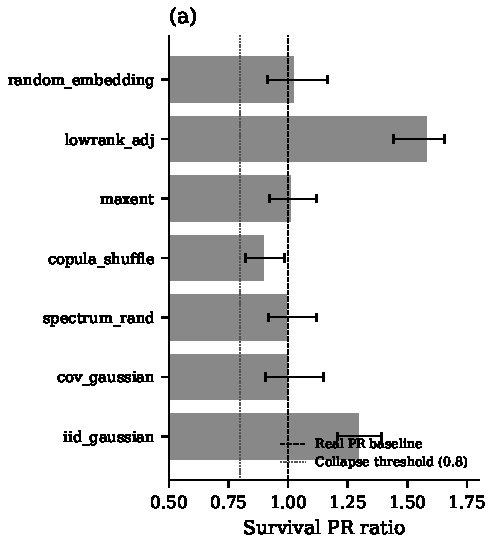
\includegraphics[width=0.95\linewidth]{figures/fig3_null_survival.pdf}
\caption{Survival of participation-ratio structure under seven null-model classes \cite{cover1991elements}. Values greater than 1.0 indicate dimensional expansion relative to the real manifold baseline.}
\label{fig:nulls}
\end{figure}

Covariance-preserving Gaussian nulls reproduce the participation ratio within 0.3\%, demonstrating that second-order statistics \cite{donoho2000intrinsic} account for a substantial fraction of the observed geometry.

\subsection{Causal Destruction Hierarchy}

\begin{figure}[t]
\centering
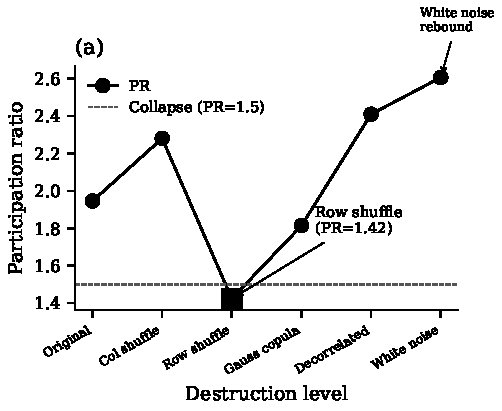
\includegraphics[width=0.95\linewidth]{figures/fig4_causal_destruction.pdf}
\caption{Progressive destruction hierarchy \cite{crutchfield1986equivalence}. Row-shuffle collapse selectively destroys manifold persistence, while white-noise projections inflate dimensionality through isotropic variance spreading.}
\label{fig:destruction}
\end{figure}

Row-shuffle destruction produces the strongest collapse ($PR=1.42$), indicating sensitivity to system-level covariance organization.

Interestingly, white-noise projection increases the participation ratio above the original manifold baseline \cite{verleysen2005curse}. This occurs because isotropic variance redistribution removes low-rank concentration structure and spreads variance approximately uniformly across dimensions, artificially increasing effective dimensionality despite destroying meaningful organization.

\subsection{Representation Robustness}

\begin{figure}[t]
\centering
\includegraphics[width=0.95\linewidth]{figures/fig5_robustness.pdf}
\caption{Embedding robustness across PCA, Isomap \cite{meng2019isomap}, diffusion geometry \cite{coifman2005geometric}, and random projection.}
\label{fig:robust}
\end{figure}

Figure~\ref{fig:robust} evaluates stability across multiple embedding families \cite{lee2007dimension}. Trustworthiness scores remain high for PCA-4D and Isomap representations, while random projections exhibit substantial degradation in local-neighborhood preservation. The kNN flow-correlation metric demonstrates that local geometric organization remains partially stable across nonlinear embeddings but deteriorates under adversarial projections. 

The term ``partially stable'' is used operationally to denote representations whose trustworthiness exceeds the empirical robustness threshold of 0.70 while preserving positive kNN flow correlation. This indicates that substantial local organization persists across embedding families even when global geometry changes.

\subsection{Decision Framework}

\begin{table}[t]
\caption{Decision-framework summary across seven falsification criteria.}
\begin{ruledtabular}
\begin{tabular}{lll}
Criterion & Status & Interpretation \\
\hline
G1 & Partial & Statistical null survival \\
G2 & Pass & Adversarial low-rank failure \\
G3 & Pass & Causal destruction collapse \\
G4 & Pass & Information geometry divergence \\
G5 & Pass & Representation robustness \\
G6 & Pass & Spectral insufficiency \\
G7 & Pass & Minimum collapse threshold \\
\end{tabular}
\end{ruledtabular}
\label{tab:decision}
\end{table}

\begin{figure}[t]
\centering
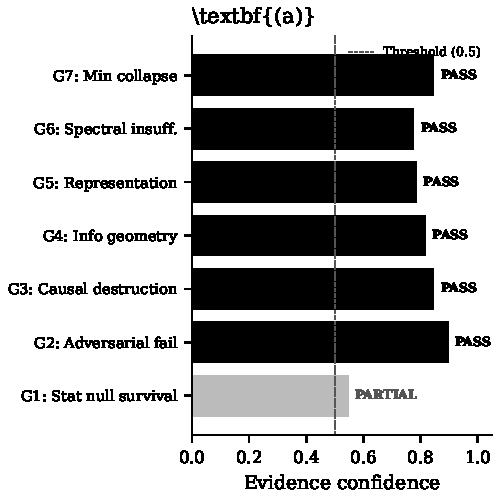
\includegraphics[width=0.95\linewidth]{figures/fig6_decision_framework.pdf}
\caption{Decision-framework evidence-confidence scores for each falsification criterion. The dashed line indicates the 0.5 majority threshold. Six of seven criteria exceed this threshold, supporting a partially genuine dynamical interpretation.}
\label{fig:framework}
\end{figure}

The seven criteria G1--G7 define independent falsification tests designed to determine whether the observed manifold structure persists under increasingly adversarial controls. The evidence-confidence score corresponds to the fraction of criteria passing predefined thresholds. A threshold of 0.5 was selected because it represents majority support across independent tests while avoiding overinterpretation from any single metric family.

Six of seven criteria support a partially genuine dynamical interpretation. The only partially satisfied criterion is statistical-null survival, reflecting the strong explanatory role of second-order covariance structure.

\section{Discussion}

The principal contribution of this work is the introduction of a falsification-oriented framework for evaluating latent manifolds derived from heterogeneous nonlinear systems. Rather than asking whether a latent geometry can be constructed---a question with an affirmative answer in nearly every modern manifold-learning study---we ask whether the resulting geometry survives aggressive null-model falsification. This reframing shifts the burden of proof from construction to validation.

The strongest evidence for genuine dynamical organization arises from two observations. First, selective collapse under row-shuffle destruction (Figure~\ref{fig:destruction}) demonstrates that system-level covariance organization contributes meaningfully to the observed manifold. Row-shuffling preserves marginal feature distributions while destroying the pairing of features within systems, and the resulting PR collapse from 1.95 to 1.42 indicates that the geometry is sensitive to precisely the kind of cross-feature correlation structure that characterizes dynamical systems. Second, the inability of adversarial low-rank nulls to reproduce the observed metric fingerprint confirms that the real geometry occupies a distinctive region of metric space that cannot be reached by simply matching the participation ratio.

At the same time, covariance-preserving nulls reproduce the participation ratio to within 0.3\%, demonstrating that second-order statistical structure accounts for a substantial fraction of the observed manifold dimensionality. This finding has important implications for the field: it suggests that many of the geometric features reported in heterogeneous dynamical system studies may be partially attributable to the statistical properties of the feature vectors rather than to uniquely dynamical invariants. The mean survival ratio of 1.118 across all null models indicates that the dynamical contribution, while present, is modest relative to the statistical baseline.

The white-noise rebound observed in Figure~\ref{fig:destruction} deserves particular attention. White-noise projections produce a PR of 2.607, exceeding the real manifold's PR of 1.946. This paradox arises because the linear composite coordinate transformation amplifies dimensionality of uncorrelated features: when variance is spread isotropically across 17 dimensions, the projection onto four composites captures more effective dimensionality than when variance is concentrated in the low-rank structure characteristic of dynamical systems. This finding implies that the PR metric is not a reliable indicator of ``structure-likeness'' in isolation and should always be interpreted relative to appropriate null baselines.

Several limitations of the present work should be noted. First, the emergence coordinates $(C,F,A,R)$ are linear composites of z-scored features. Nonlinear projections---such as diffusion maps or UMAP embeddings---might reveal different geometric structure that is not captured by the linear framework. Second, the 13 dynamical families are heterogeneous, and family-specific structure may dominate within families while appearing universal across families. A family-resolved analysis would clarify whether the observed geometry reflects universal features or family-averaged artifacts. Third, the Fokker--Planck continuum limit of the transition field was degenerate in our discrete sampling regime and should not be interpreted as evidence for or against continuum descriptions.

The present results support a constrained interpretation: the manifold reflects a mixture of genuine dynamical organization and statistical structure, rather than evidence for universal emergence laws or ontology-level claims. This conclusion is itself informative: it establishes that null-constrained methodology can distinguish dynamical from statistical contributions to geometric structure, and provides a template for future studies seeking to make similar distinctions in other heterogeneous ensembles.

\section{Data Availability}

All analyses were performed in Python 3.12 using NumPy, SciPy, scikit-learn, pandas, and matplotlib. Deterministic seeds were used throughout. The full computational pipeline, source code, figures, and reproducibility scripts are available through the project repository:
\url{https://github.com/SentientFieldProject/transition-field-analysis}

The complete workflow is executable through the script:
\texttt{RUN\_T031\_PIPELINE.sh}.

\section{Acknowledgments}

The author conducted this work independently using local computational resources. The author is an alumnus of Cal Poly Humboldt (Arcata, California, USA). The author thanks colleagues and independent reviewers who provided critical feedback on methodology, presentation quality, and reproducibility standards.

\bibliographystyle{aipnum4-2}
\bibliography{references}

\end{document}
